\documentclass[conference]{IEEEtran}
\IEEEoverridecommandlockouts
% The preceding line is only needed to identify funding in the first footnote. If that is unneeded, please comment it out.
\usepackage{cite}
\usepackage{amsmath,amssymb,amsfonts}
\usepackage{algorithmic}
\usepackage{graphicx}
\usepackage{textcomp}
\usepackage{authblk}
\usepackage{array}
\usepackage{indentfirst}
\usepackage{afterpage}
\usepackage{caption}
\usepackage{subcaption}
\def\BibTeX{{\rm B\kern-.05em{\sc i\kern-.025em b}\kern-.08em
    T\kern-.1667em\lower.7ex\hbox{E}\kern-.125emX}}

\begin{document}

\title{\huge A Generator Supporting Data Abstraction in GPU Kernels}

\author{Derek Rayside}
\author{Steven Stewart}
\author{Di Sen Lu}
\author{Zhao Tian Fang}
\author{Cheng Dong}
\author{Andrew Zhou}
\author{Zu Qi Li}
\author{Clement Hoang}

\renewcommand\Authands{ and }

\affil{Electrical \& Computer Engineering, University of Waterloo}
\affil{drayside@uwaterloo.ca} 

\maketitle

\begin{abstract}
Optimizing a GPU kernel often involves re-arranging how it accesses memory. Finding the best arrangement can be difficult and time-consuming, and might vary from chip to chip. Data abstraction is a program structuring technique for separating the logical operations of the program from the physical arrangement of the underlying memory. Existing GPU kernel APIs have limited support for data abstraction, and so kernel optimization often requires rewriting significant parts of the kernel when the physical memory organization has been changed, even though the logical operation of the kernel remains the same. This paper presents an embedded DSL and associated generator that provides some data abstraction for GPU kernels. On both the host (CPU) and device (GPU) side, the programmer writes in terms of the abstract logic of the program. Configuration parameters control how the logical memory is mapped to physical memory. The provided abstraction mechanisms support data prefetching, data packing, and encoding two-dimensional data into one-dimensional data.
\end{abstract}

\section{Introduction}
Optimizing a GPU kernel code is largely about making machine-oriented decisions. These machine-oriented decisions can require significant changes to the kernel code, making it difficult to experiment with different decisions. We present an embedded DSL and an associated code generator that encapsulate a number of machine-oriented decisions in GPU kernels, making the logical organization of the kernel more obvious and experimentation easier. 

Our embedded DSL and generator encapsulate three machine-oriented decisions: copying data from GPU-global memory to GPU-local memory - which we name prefetching; packing multiple logical values into a single physical array cell; and encoding two-dimensional data into various one-dimensional representations.

The key ideas are old ones: information hiding [9] and data abstraction [4, 7]. Yet it appears that in this context they have either been applied in extreme, as new high languages that insulate the programmer from almost all machine-oriented decisions, or hardly at all in low-level languages that focus on the machine at the expense of other concerns. The combination of an embedded DSL on the host (CPU) side and generated code on the device (GPU) side seems to hit a middle-ground on this spectrum.

\section{Techniques}
On the host (CPU) side we present a library to provide abstractions for common memory operations such as transferring data to and writing data from the device (GPU). Configurations are set on the host side for arrays to perform any combination of the three machine-oriented decisions. On the device (GPU) side, the generated code provides the programmer with a uniform interface to the logical organization of the data. The kernel code written by the programmer remains the same even when the host side configuration is changed. The current implementation is C++ on the host side, generating OpenCL code on the device side.

The main class on the host is Mem, which represents a memory (array) that is shared between the CPU and the GPU. The Mem class is configured by a MemCapacity object and a MemConfig object. A MemCapacity object specifies how much space is allocated on both the host side and the device side. This specification could be statically fixed or indicate that the value will be set dynamically. The MemConfig object specifies the configuration for performing machine-oriented decisions. \\
The generator produces initialization, accessor and mutator operations for each Mem object. The names of these operations are prefixed with the name of the specific Mem object, so that each Mem can be individually configured. 


\subsection{Packing}
The MemConfig object specifies the maximum number of bits used for each value in Mem. Mem packs multiple logical values into 32 bit physical storage. If all elements in an array are known to take x bits, then we can fit 32/x elements inside a 32 bit cell. 

The generated accessor and mutator operations on the kernel handle translating logical indices into physical cells and then packing and unpacking the data, if necessary. 

Writing to packed data requires additional concurrency control, since multiple logical values share a physical cell, but the write must be to the entire physical cell. The generated mutator code for packed arrays incorporates a lock-free loop using atomic operations. First, the physical cell is read to a local variable; then the logical value is changed in this local variable; finally, an atomic compare-and-swap writes the new cell value back to the array if the value in the array has not been mutated by another thread. The loop repeats until the write is successful. Kernels that perform many write operations to logical indices that are packed into the same cell might experience a runtime slowdown as these writes are effectively serialized (whereas they might have occurred in parallel if the data were not packed). Packing is generally recommended for kernel inputs rather than outputs.

\subsection{Prefetching}
The MemConfig object also specifies whether the data are to be prefetched from GPU global memory to GPU local memory before the kernel computation occurs. In the kernel code, the amount of data to be prefetched, and its offset in the global array with respect to the logical indices, are indicated by the programmer. Prefetching can be applied to both one-dimensional and two-dimensional arrays. The local memory prefetched is automatically converted to physical cell addresses when packing is enabled.

Prefetching is invoked through a generated initialization operation. This is decomposed into potentially two loops, depending on whether the number of cells in the array is a multiple of the workgroup size. The first loop has the most iterations, and prefetches up to the largest multiple of the workgroup size that is less than or equal to the number of cells to be prefetched. This first loop does not include a conditional in the body. The second loop prefetches the remainder of the cells, and must include a conditional to ensure that the prefetch does not go off the end of the arrays. Conditionals are discouraged in GPU kernels because they might cause thread divergence: i.e., different threads computing different instructions. The SIMD data-parallel model of most GPU chips requires that every thread in a workgroup execute the same instructions, and so if divergence occurs all threads execute both branches and then discard the results of the other branch. The aim of separating the prefetch into these two loops is to reduce potential divergence.

\subsection{Memory Encoding}
The MemConfig object specifies how two-dimensional data used in the kernel code are represented in one-dimension. Two-dimensional arrays are categorized into two types: rectangular arrays and variable length arrays. Rectangular arrays contain rows of uniform length whereas variable length arrays have rows of varying length. For rectangular arrays, there is one major decision: row-major or column-major form.

When the rows are of varying length, the one-dimensional array can be encoded in many ways. One way is to divide the variable length array into multiple arrays each having rows of uniform length. We denote each array as a page and invoke multiple kernel launches for each page. Since each page is a rectangular array, the decision becomes row-major or column-major as shown in Figure 4.d.

The variable length two-dimensional array can also be kept as a single page (array). One encoding method is to pad the rows out to a standard (maximum) length. This way, we can again perform row-major or column-major transformations shown in Figure 4.a.

The second encoding method is to append each row to the end of the previous row in row-major format. A special symbol called the delimiter is placed between each row to indicate where it starts as shown in Figure 4.b.
Another encoding method is to also append each row to the end of the previous row in row-major format, but also uses a separate array, called offset array to track rows. The offset array contains the indices of the start of each row as shown in Figure 4.c. In summary:

\begin{center}
\begin{tabular}{ | m{3em} | m{3cm}| m{3cm} | } 
\hline
 & Row-Major & Column-Major \\ 
\hline
Single page & \begin{tabular}{@{}c@{}}Padding \\ Offset array \\ Delimiters \end{tabular} & Padding \\ 
\hline
Multiple pages & No padding & No padding \\ 
\hline
\end{tabular}
\end{center} 
    
The generated accessor and mutator operations on the kernel access the one-dimensional array using the corresponding two-dimensional array interface. This makes the kernel more readable and allows programmers focus on the logical components rather than the underlying physical one-dimensional representation. Memory is automatically accessed from local memory when prefetching is enabled. The elements in the two-dimensional array are also automatically converted to physical cell addresses when packing is enabled.

\section{Experiments}
Figure 1, 2, 3 presents some comparative times on three different GPU cards; an Intel Iris 6100 in a MacBook Air laptop; an Nvidia GeForce GTX 950 (a mid-range desktop GPU); and a Nvidia Tesla P4 (top of the line workstation GPU).

The plots in Figure 1, 2, 3 measure kernel compute time in the left column and upload latency in the right column. Upload latency is the time it takes to copy the data from the host (CPU) memory to the device (GPU) memory.

The results show that packing, prefetching and memory encoding can all have some impact on kernel performance, and that this impact varies by hardware. With prefetching and memory encoding the benefits are primarily in compute times, whereas the benefit of packing is in reduced upload latency. While packing can reduce upload latency, it does not appear to negatively affect compute times. For variable length arrays, different memory encodings impact both compute times and upload latency.

\subsection{Packing 2-bit values}
This experiment calculates the sum of all the values in a large input array of 2-bit values. The first kernel receives the values as packed integers, with 16 values being stored in a single 32-bit integer, while the second kernel receives them as unpacked integers, with only one value in a 32-bit integer. The size of the input array is 16 times larger in the unpacked case.

Figure 1 shows that packing results in a significant upload latency improvement on the Intel Iris 6100 and the Tesla P4, and a modest improvement on the GTX 950. Figure 1 also shows that packing does not impede compute times on any of the cards, even though unpacking the data requires more instructions.

\subsection{Prefetching inputs to local memory}
The GPU memory hierarchy must be explicitly managed by the programmer. When data are copied from the host (CPU) to the device (GPU), they are copied to global memory. This is the slowest (and largest) memory on the GPU card. Each multiprocessor on the GPU card, which typically has 32 or 64 cores, has its own local memory.

A commonly recommended optimization [1] is to copy data from global memory to local memory. This optimization is most relevant when the data are to be read multiple times, or are to be read in an arbitrary order. In the latter case, the prefetch from global memory can be conducted in a coalesced manner, and then memory accesses can be from local memory.

This experiment receives an input array of 32 integer values and a large output array. There are as many work-items as there are elements in the output array. Every work-item calculates the sum of all 32 input values and stores the sum in the relevant element of the output array. The first kernel prefetches the input array into local memory and then repeatedly reads from local memory, while the second kernel works exclusively on the slower global memory.

Prefetching shows significant reduction in compute times on the P4 (Figure 1), and a modest reduction in compute time on the Intel Iris 6100 and GTX 950.


\subsection{Rectangular 2-dimensional array encoding}
This experiment copies all the values from a large input square matrix into an output matrix. The first kernel utilizes the work items to act on the matrix in row major format, while the second kernel utilizes them to act on the matrix in column major format. The second kernel encourages advantageous global memory coalescing by aligning the work items along the faster-moving X-dimension.	

Figure 1 shows that different memory encodings can have a significant impact on compute times, as expected [1].


\subsection{Variable length 2-dimensional array encoding}
This experiment is performed on a clause inspection kernel for SAT solving that use variable length 2-dimensional arrays. The kernel receives an array of clauses (clause database) each composing of literals. The kernel also receives an assignment array that maps literals to boolean values. The first kernel receives a dense clause database containing a million clauses, each clause consisting of 80-100 literals. Figure 2 shows that column-major padding has better compute times across all three devices than the other encodings. Multi-page encoding has smaller upload latency for Intel Iris and GTX 950, but not for Tesla P4. However, unlike multi-page, row-major padding, column-major padding and offset array have higher upload latencies due to space inefficiency.

The second kernel receives a sparse clause database containing a million clauses, each clause consisting of 10-100 literals. Figure 3 shows that row-major padding, column-major padding and offset array have better compute times across all three devices. Multi-page does has a high upload latency with sparse data because of the overhead of initializing multiple kernel launches. Offset array however, has the smallest upload latency across all three devices due to space efficiency. Row-major padding, column-major padding and offset array have varied compute times across different devices.

The delimiter array compute and upload latency times are not shown in Figure 2 and 3 because this encoding technique performs very inefficiently. This technique has a linear time complexity for array access, which results in extremely slow computations. In summary:

\begin{center}
\begin{tabular}{ | m{5em} | m{3cm}| m{3cm} | } 
\hline
 & Advantages & Disadvantages \\ 
\hline
Row/column major padding & Fast compute times with dense input. Padding supports coalesced reads and writes, improving compute times & High upload latency with sparse input \\ 
\hline
Offset array & Small upload latency with sparse input & Higher upload latency due to offset array
and slower compute time due to extra lookup in offset array \\ 
\hline
Multi-page & Small upload latency with dense input. Rectangular data supports coalesced reads and writes, improving compute times & High upload latency with sparse input. Lose track of row ordering in original matrix \\ 
\hline
Delimiters & N/A & N/A \\ 
\hline
\end{tabular}
\end{center} 

While the experiments were performed on a kernel intended for SAT solving, this library may not necessarily improve an existing GPU-based SAT solver. These memory encoding techniques for variable length arrays show that memory encoding vary between hardware and that it is important to consider different techniques in different circumstances.

\section*{Related Work}
Our work exists in somewhere in the middle of the hardware- specific vs. usability spectrum of GPU programming technologies. At one extreme, the HSA (Heterogeneous System Architecture) Intermediate Language (HSAIL) [5] has several pre-defined packings for arrays. The smallest logical values that can be packed are 8 bits, which can be packed into 32, 64, or 128 bit physical values. HSAIL is an assembler-like language that is intended to be produced by compilers, not written by people.
					
At the other extreme, new programming languages like Brook [2] and Single-Assignment C (SAC) [3] provide unifying data abstractions (streams or arrays, respectively) and insulate the programmer from the hardware. To our knowledge, neither support array packing or prefetching; both appear to automatically assign work dimensions.
					
OpenCL [6] is a portable subset of C99 for GPU programming. While usable, it is intended to give the programmer control over the hardware. OpenCL has a packed attribute for structs, but this does not apply to arrays. OpenCL also has some predefined packings for images, where the RGB values are encoded in different bit-ranges of a 32 bit int [6]. OpenCL is the target language of our code generator.

\section*{Conclusion}
GPU kernel programming is typically a machine-oriented exercise. We present a host-side embedded DSL and associated device-side code generator that provide some abstractions to some machine-oriented decisions, such as whether to pack arrays, whether to prefetch data, and how to encode two-dimensional data into one-dimensional data. 

These abstractions facilitate the programmer writing the kernel code itself in terms of the logical organization of the data, even though the physical arrangement of the data on the hardware might change. This can make the kernel code easier to understand and maintain.

These abstractions also allow the programmer to automatically adjust parameters based on the hardware available at runtime. These hardware-oriented decisions can now be controlled by flipping configuration bits, without having to change any of the hand-written code.

\begin{thebibliography}{00}
\bibitem{b1} AMD Inc. AMD Accelerated Parallel Processing OpenCL Optimization Guide, 2014.
\bibitem{b2} I. Buck, T. Foley, D. Horn, J. Sugerman, K. Fatahalian, M. Houston, and P. Hanrahan. Brook for GPUs: stream computing on graphics hardware. ACM Transactions on Graphics, 23(3):777-786, 2004.
\bibitem{b3} Clemens Grelck and Sven-Bodo Scholz. SAC: A Function- alArray Language for Efficient Multi-threaded Execution. International Journal of Parallel Programming, 34(4), 2006.
\bibitem{b4} C. A. R. Hoare. Proof of correctness of data representations. Acta Informatica, 1(4):271-281, 1972.
\bibitem{b5} HSA Foundation. HSA Programmer's Reference Manual: HSAIL Virtual ISA and Programming Model, Compiler Writer?s Guide, and Object Format (BRIG), 2013. Document \#49828, rev. 0.95.
\bibitem{b6} Khronos Group. OpenCL Specification v1.1, 2011.
\bibitem{b7} Barbara H. Liskov. Data abstraction and hierarchy. In Nor- man K. Meyrowitz, editor, OOPSLA, Orlando, FL, 1987. URL http://doi.acm.org/10.1145/62138.62141.
\bibitem{b8} Sparsh Mittal and Jeffrey Vetter. A Survey of CPU-GPU Heterogeneous Computing Techniques. ACM Computing Surveys, 2015.
\bibitem{b9} David Lorge Parnas. On the Criteria to be Used in Decomposing Systems into Modules. CACM, 15(12):1053-1058, 1972.
\end{thebibliography}

\clearpage
\newpage

\begin{figure}
\centering
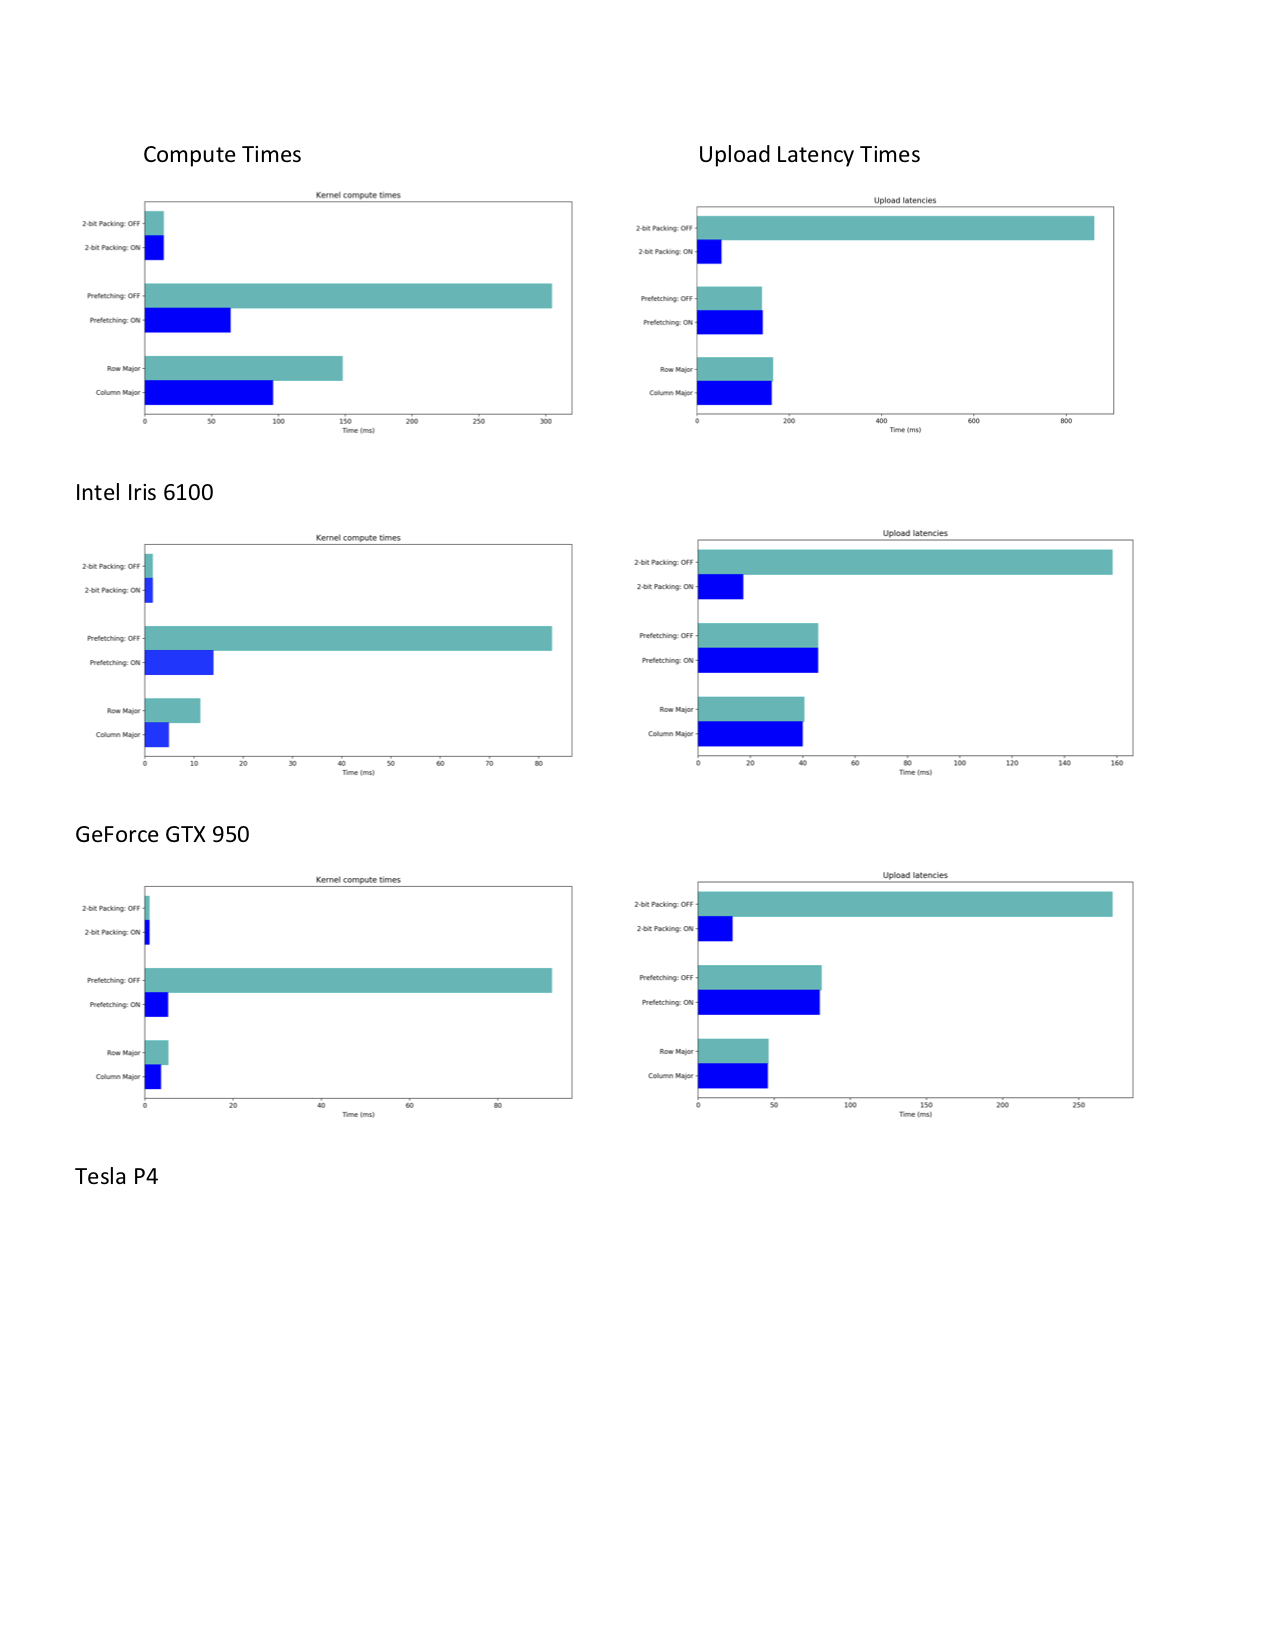
\includegraphics[scale=0.45]{misc_data.jpg}
\caption{Data from rectangular arrays. Compute (left) and upload latency (right) times. Shorter is better.}
\end{figure}

\clearpage
\newpage

\begin{figure}
\centering
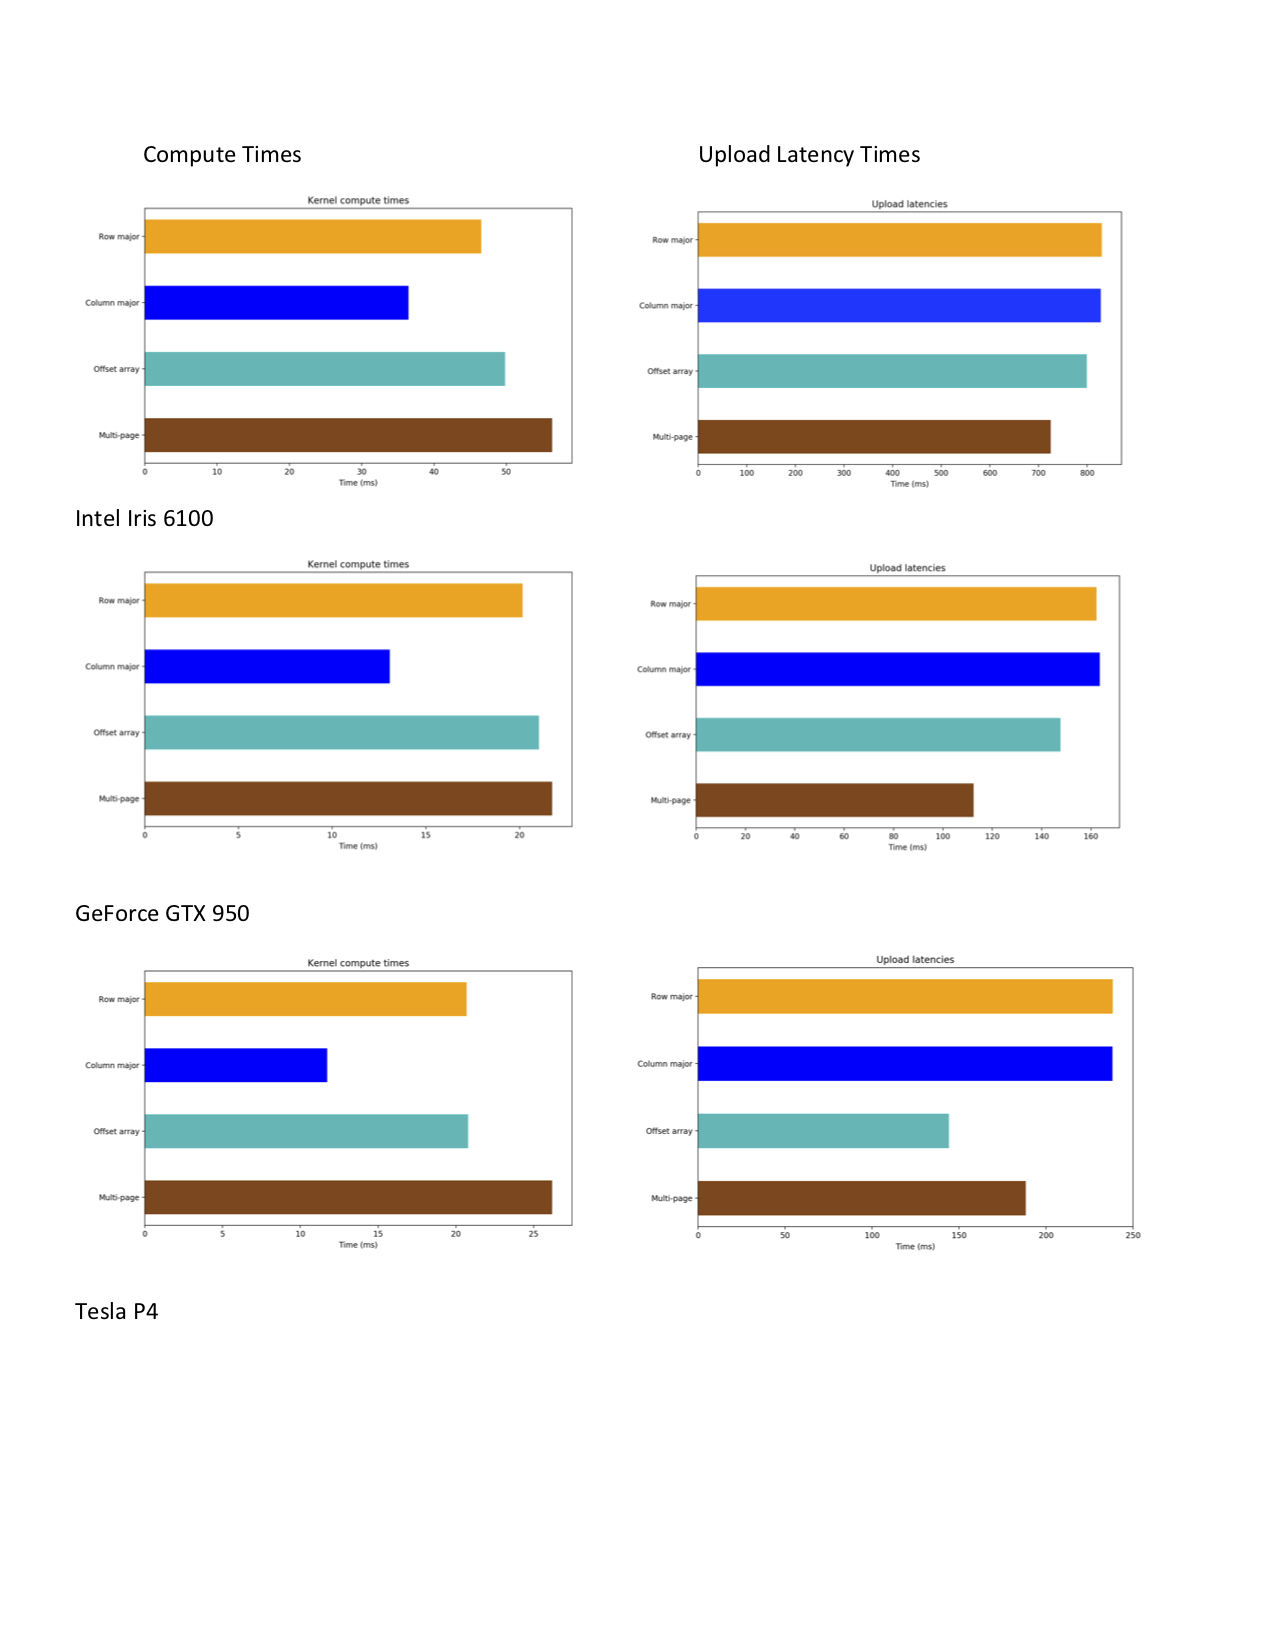
\includegraphics[scale=0.45]{var_dense.jpg}
\caption{Dense variable length arrays. Compute (left) and upload latency (right) times. Shorter is better.}
\end{figure}

\clearpage
\newpage

\begin{figure}
\centering
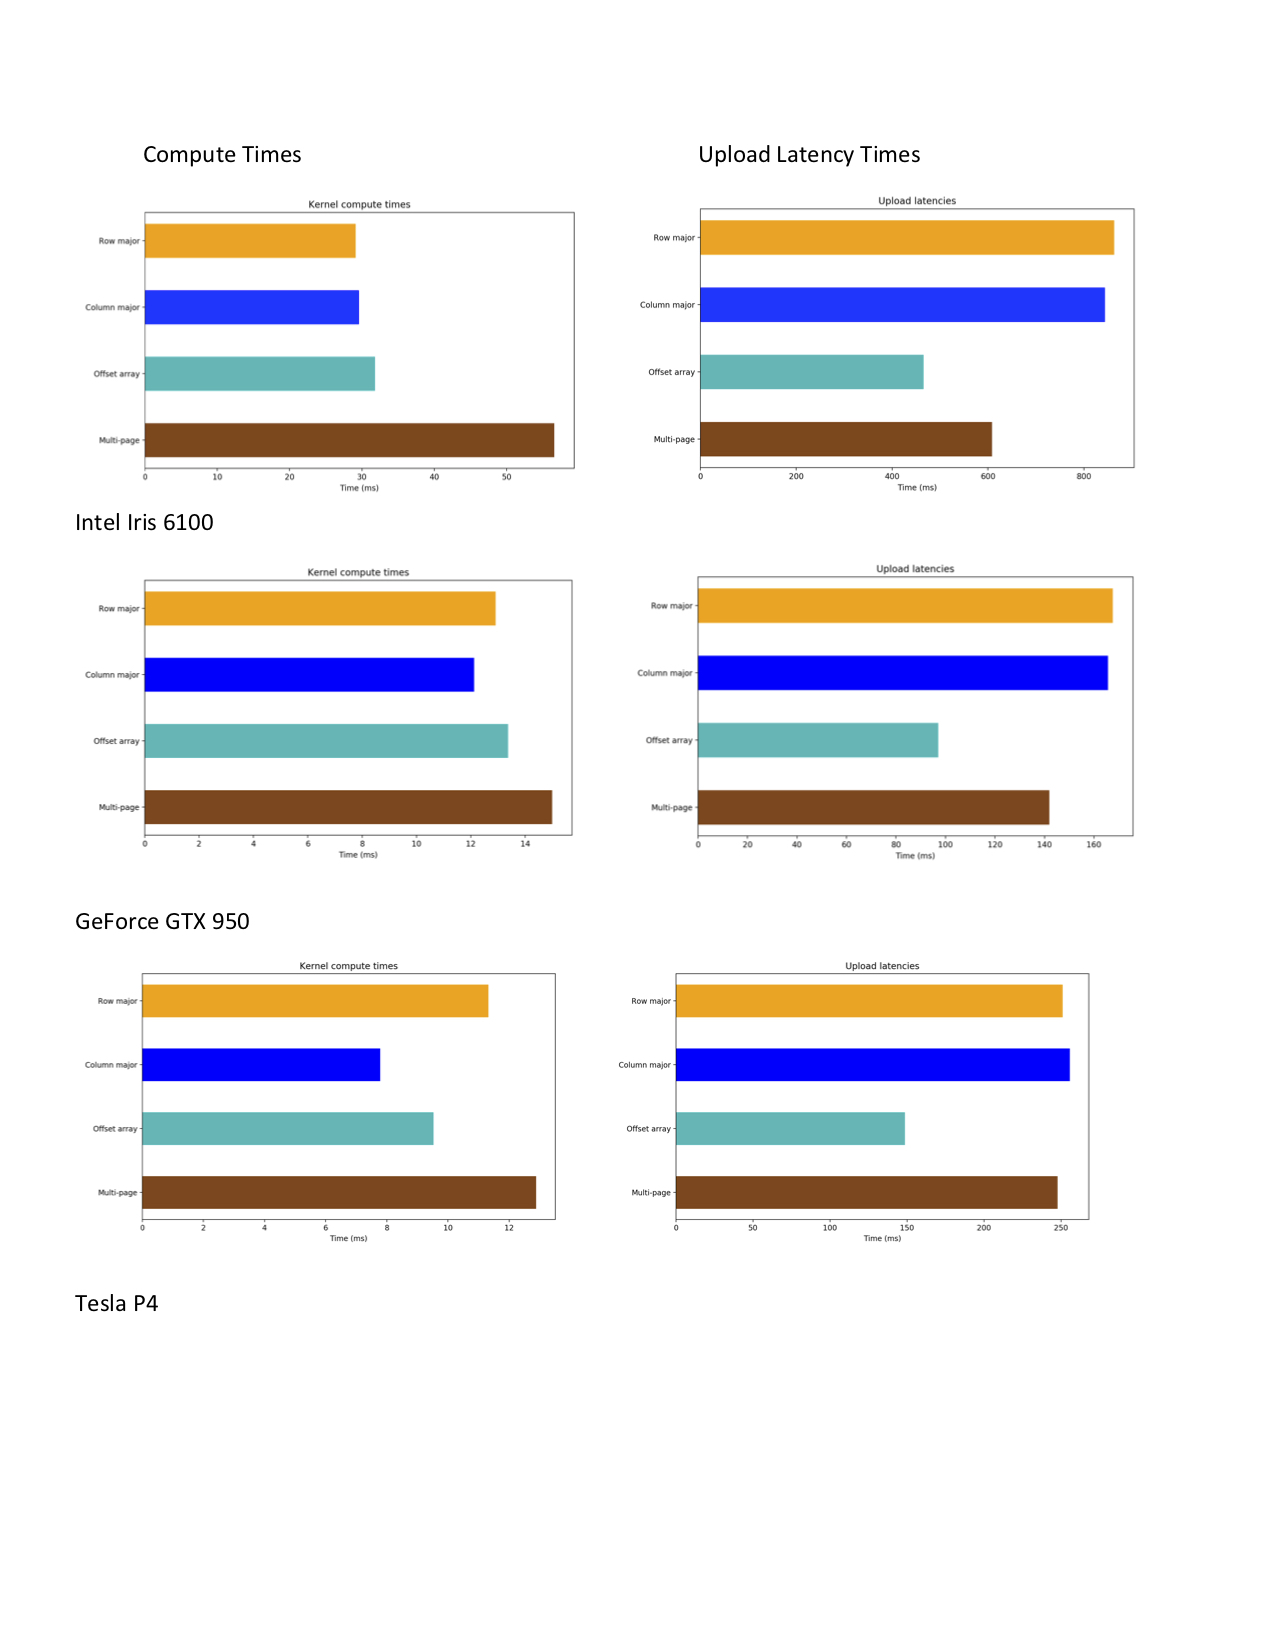
\includegraphics[scale=0.45]{var_sparse.jpg}
\caption{Sparse variable length arrays. Compute (left) and upload latency (right) times. Shorter is better.}
\end{figure}

\clearpage
\newpage

\begin{figure}
\centering
\begin{subfigure}[b]{0.3\textwidth}
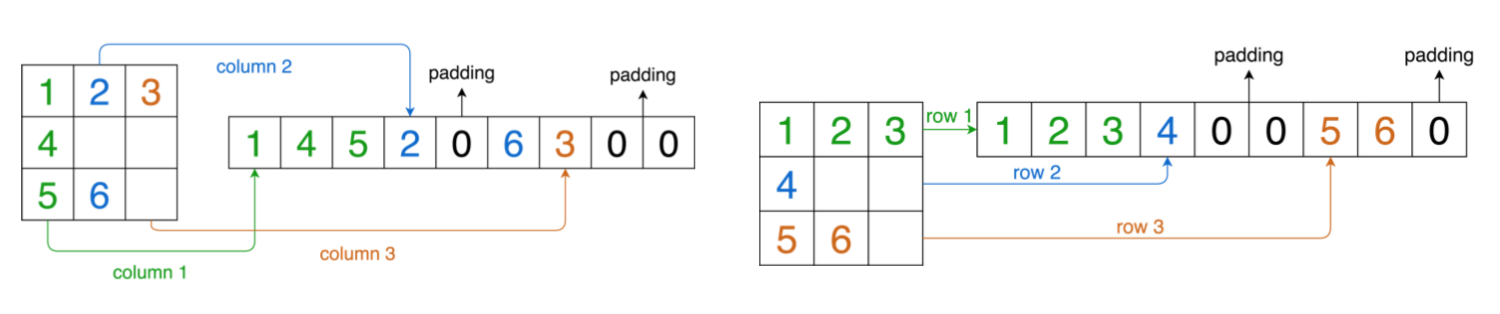
\includegraphics[scale=0.6]{padding.png}
\caption{Column-major padding (right) and row-major padding (left)}
\end{subfigure}
\begin{subfigure}[b]{0.3\textwidth}
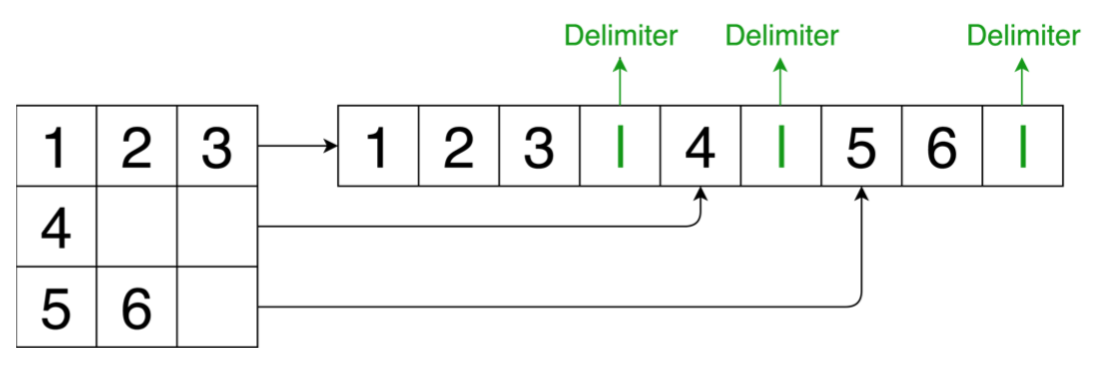
\includegraphics[scale=0.5]{delimiter.png}
\caption{Delimiter technique}
\end{subfigure}
\begin{subfigure}[b]{0.3\textwidth}
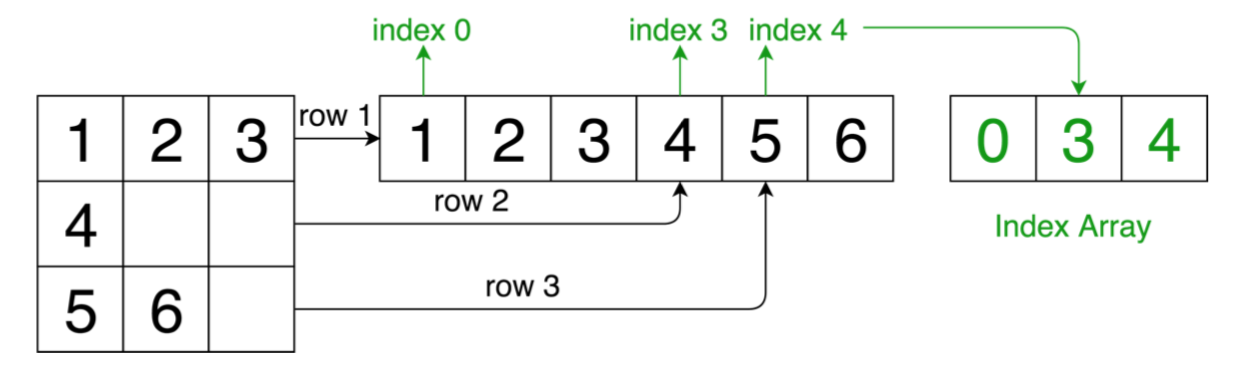
\includegraphics[scale=0.5]{offset.png}
\caption{Offset array}
\end{subfigure}
\begin{subfigure}[b]{0.3\textwidth}
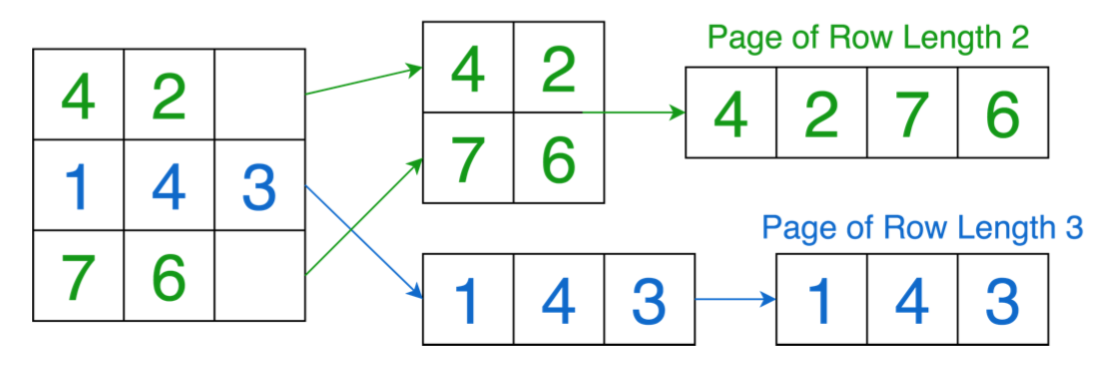
\includegraphics[scale=0.5]{multipage.png}
\caption{Multi-page technique}
\end{subfigure}
\caption{Variable length array encodings}
\end{figure}



\end{document}
